\lecture{9}{Feb 26 01:10}{}

\section*{Finite Square Well (FSQ) Notes}

\noindent
\textbf{Potential Setup:}
\[
V(x) = 
\begin{cases}
V_0, & x < -\frac{a}{2},\\[6pt]
0,    & -\frac{a}{2} \le x \le \frac{a}{2},\\[6pt]
V_0, & x > \frac{a}{2}.
\end{cases}
\]
We assume $V_0 > 0$ and define the well to extend from $-\tfrac{a}{2}$ to $+\tfrac{a}{2}$. We want to solve the time‐independent Schr\"odinger equation,
\[
\hat{H}\,\psi_n(x) \;=\; E_n\,\psi_n(x), 
\quad
\hat{H} \;=\; -\frac{\hbar^2}{2m}\,\frac{d^2}{dx^2} \;+\; V(x).
\]
The full time‐dependent wavefunction can be written as $\psi(x,t) = \psi_n(x)\,e^{-\tfrac{i E_n t}{\hbar}}$.

\medskip
\noindent
\textbf{Two energy regimes:}
\begin{itemize}
\item $E > V_0$
\item $E < V_0$
\end{itemize}
Both cases lead to piecewise solutions (exponential vs.\ oscillatory) in the outer regions depending on whether $E < V_0$ or $E > V_0$.

\section*{Case: $E < V_0$}
\subsection*{Region I: $x < -\frac{a}{2}$ (where $V=V_0$)}
The Schr\"odinger equation in Region~I is
\[
-\frac{\hbar^2}{2m}\,\frac{d^2}{dx^2}\,\psi_n(x) \;+\; V_0\,\psi_n(x)
\;=\;
E_n\,\psi_n(x).
\]
Rearrange to
\[
-\frac{\hbar^2}{2m}\,\frac{d^2}{dx^2}\,\psi_n(x)
\;=\;
\bigl(E_n - V_0\bigr)\,\psi_n(x).
\]
Since $E_n < V_0$, define
\[
\kappa \;=\; \sqrt{\frac{2m\bigl(V_0 - E_n\bigr)}{\hbar^2}},
\]
so the equation becomes
\[
\frac{d^2}{dx^2}\,\psi_n(x) = \kappa^2\,\psi_n(x).
\]
The general solution is
\[
\psi_n^{(I)}(x) \;=\; A\,e^{\,\kappa\,x} \;+\; B\,e^{-\kappa\,x}.
\]
But as $x\to -\infty,$ we must avoid an unbounded solution; hence typically we set
\[
\psi_n^{(I)}(x) \;=\; A\,e^{\,\kappa\,x} \quad\text{(assuming the $e^{-\kappa x}$ term blows up).}
\]

\subsection*{Region II: $-\,\frac{a}{2} \le x \le \frac{a}{2}$ (where $V=0$)}
Here,
\[
-\frac{\hbar^2}{2m}\,\frac{d^2}{dx^2}\,\psi_n(x) = E_n\,\psi_n(x).
\]
Define
\[
k \;=\; \sqrt{\frac{2m E_n}{\hbar^2}}.
\]
The general solution is
\[
\psi_n^{(II)}(x)
\;=\;
C\,\cos\bigl(k\,x\bigr) \;+\; D\,\sin\bigl(k\,x\bigr).
\]

\subsection*{Region III: $x > \frac{a}{2}$ (where $V=V_0$)}
Same form as Region~I:
\[
-\frac{\hbar^2}{2m}\,\frac{d^2}{dx^2}\,\psi_n(x)
\;=\;
\bigl(E_n - V_0\bigr)\,\psi_n(x)
\;=\; -\bigl(V_0 - E_n\bigr)\,\psi_n(x),
\]
with the same $\kappa$ as above.  The general solution is
\[
\psi_n^{(III)}(x) \;=\; F\,e^{\,\kappa\,x} + G\,e^{-\kappa\,x}.
\]
But for $x\to +\infty$, finiteness requires $e^{\,\kappa x}$ must vanish, so typically
\[
\psi_n^{(III)}(x) = G\,e^{-\kappa\,x}.
\]

\medskip
\noindent
\textbf{Boundary conditions:}  
We require continuity of $\psi_n(x)$ and of its derivative $\psi_n'(x)$ at $x=\pm \tfrac{a}{2}$.  These lead to transcendental equations that determine the allowed energies $E_n$.  

\begin{figure}[h!]
\centering
\setlength{\unitlength}{1mm}
\begin{picture}(80,35)
\put(0,0){\line(1,0){80}}
\put(20,0){\line(0,1){20}}
\put(60,0){\line(0,1){20}}
\put(20,20){\line(1,0){40}}
\put(10,23){\makebox(0,0){$V_0$}}
\put(40,10){\makebox(0,0){Well region}}
\put(65,10){\makebox(0,0){$x$}}
\put(19,-3){\makebox(0,0){$-\tfrac{a}{2}$}}
\put(61,-3){\makebox(0,0){$\tfrac{a}{2}$}}
\end{picture}
\caption{Finite square well with width $a$ and height $V_0$.}
\end{figure}

\section*{Even/Odd (Symmetric/Antisymmetric) Solutions}
Because the potential is symmetric about $x=0$, we can classify solutions by parity:
\[
\hat{P}\,\psi_n(x) \;=\; \psi_n(-x) \;=\; \pm\,\psi_n(x).
\]
Thus we look for either \emph{even} solutions ($+$ sign) or \emph{odd} solutions ($-$ sign).

\paragraph{Even solutions.} 
An \emph{even} wavefunction means
\[
\psi_n(-x) = \psi_n(x).
\]
In Region II, an even solution can be taken in the form
\[
\psi_n^{(II)}(x) \;=\; A_s\,\cos\bigl(k\,x\bigr).
\]
Matching at $x=\pm\tfrac{a}{2}$ gives conditions leading to a transcendental equation (often written as $\tan(k\,a/2)$ = \dots).

\paragraph{Odd solutions.}
An \emph{odd} wavefunction means
\[
\psi_n(-x) = -\,\psi_n(x),
\]
which in Region~II is typically
\[
\psi_n^{(II)}(x) \;=\; A_a\,\sin\bigl(k\,x\bigr).
\]
Similarly, matching the boundary conditions yields a different transcendental equation (often involving $-\cot(k\,a/2)$).

\medskip
\noindent
\textbf{Outside regions} (I and III) then get exponentials of the form $e^{\kappa x}$ or $e^{-\kappa x}$ with appropriate amplitudes chosen to preserve the even or odd symmetry (i.e.\ the same magnitude outside $\pm a/2$, possibly with a sign flip in the odd case).

\section*{Graphical Solution and Quantization Conditions}
\begin{figure}[H]
    \centering
    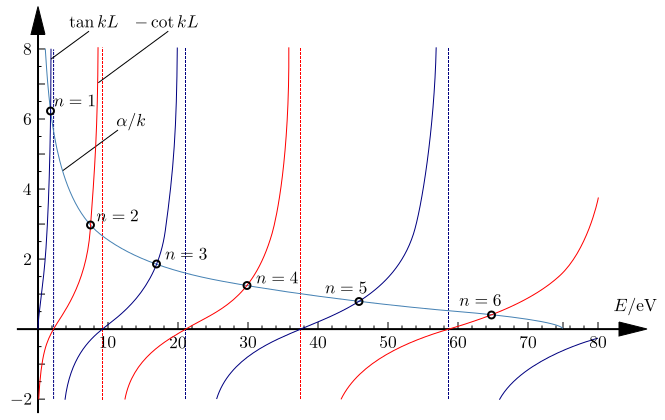
\includegraphics[width=0.6\textwidth]{Figures/06.png}
    \caption{}
    \label{fig:}
\end{figure}
By enforcing continuity of $\psi_n$ and $\psi_n'$, one arrives at equations typically written in the form:
\[
k = \sqrt{\frac{2m\,E}{\hbar^2}}, 
\quad
\kappa = \sqrt{\frac{2m\,(V_0 - E)}{\hbar^2}}.
\]
Then for \emph{even} solutions:
\[
\tan\!\bigl(k\,\tfrac{a}{2}\bigr) 
= 
\frac{\kappa}{k}, 
\]
while for \emph{odd} solutions:
\[
-\cot\!\bigl(k\,\tfrac{a}{2}\bigr) 
= 
\frac{\kappa}{k}.
\]
These transcendental equations can be solved numerically or by graphical methods.  One typically plots the left‐hand sides ($\tan$ or $-\cot$) alongside the right‐hand side $\kappa/k$ and finds the intersections that give the allowed $k$ (and hence the allowed $E$).

\bigskip
\begin{center}
\textit{As limits:} 

- If $V_0 \to \infty,$ this reduces to the \emph{infinite} square well of width $a$.\\
- If $a \to \infty,$ one recovers a \emph{free particle}.\\
- If $a \to 0$ with $V_0\,a =$ const, one can get a delta‐function‐like potential. 
\end{center}